\section{Astronomy and the Atmosphere}
\seclabel{astronomy_and_the_atmosphere}


From the very beginning, humans have surely stared into space and
contemplated its brilliance.  Stone circles in the Nabta Playa in
Egypt are likely the first observed astronomical observatory and
are believed to have acted as a prehistoric calendar.  Dating back
to the 5th century BC, they are 1,000 years older than stonehenge
\citep{mck-mahille_2007_astronomy-nabta}.

\begin{figure}[htbp]
  \centering
  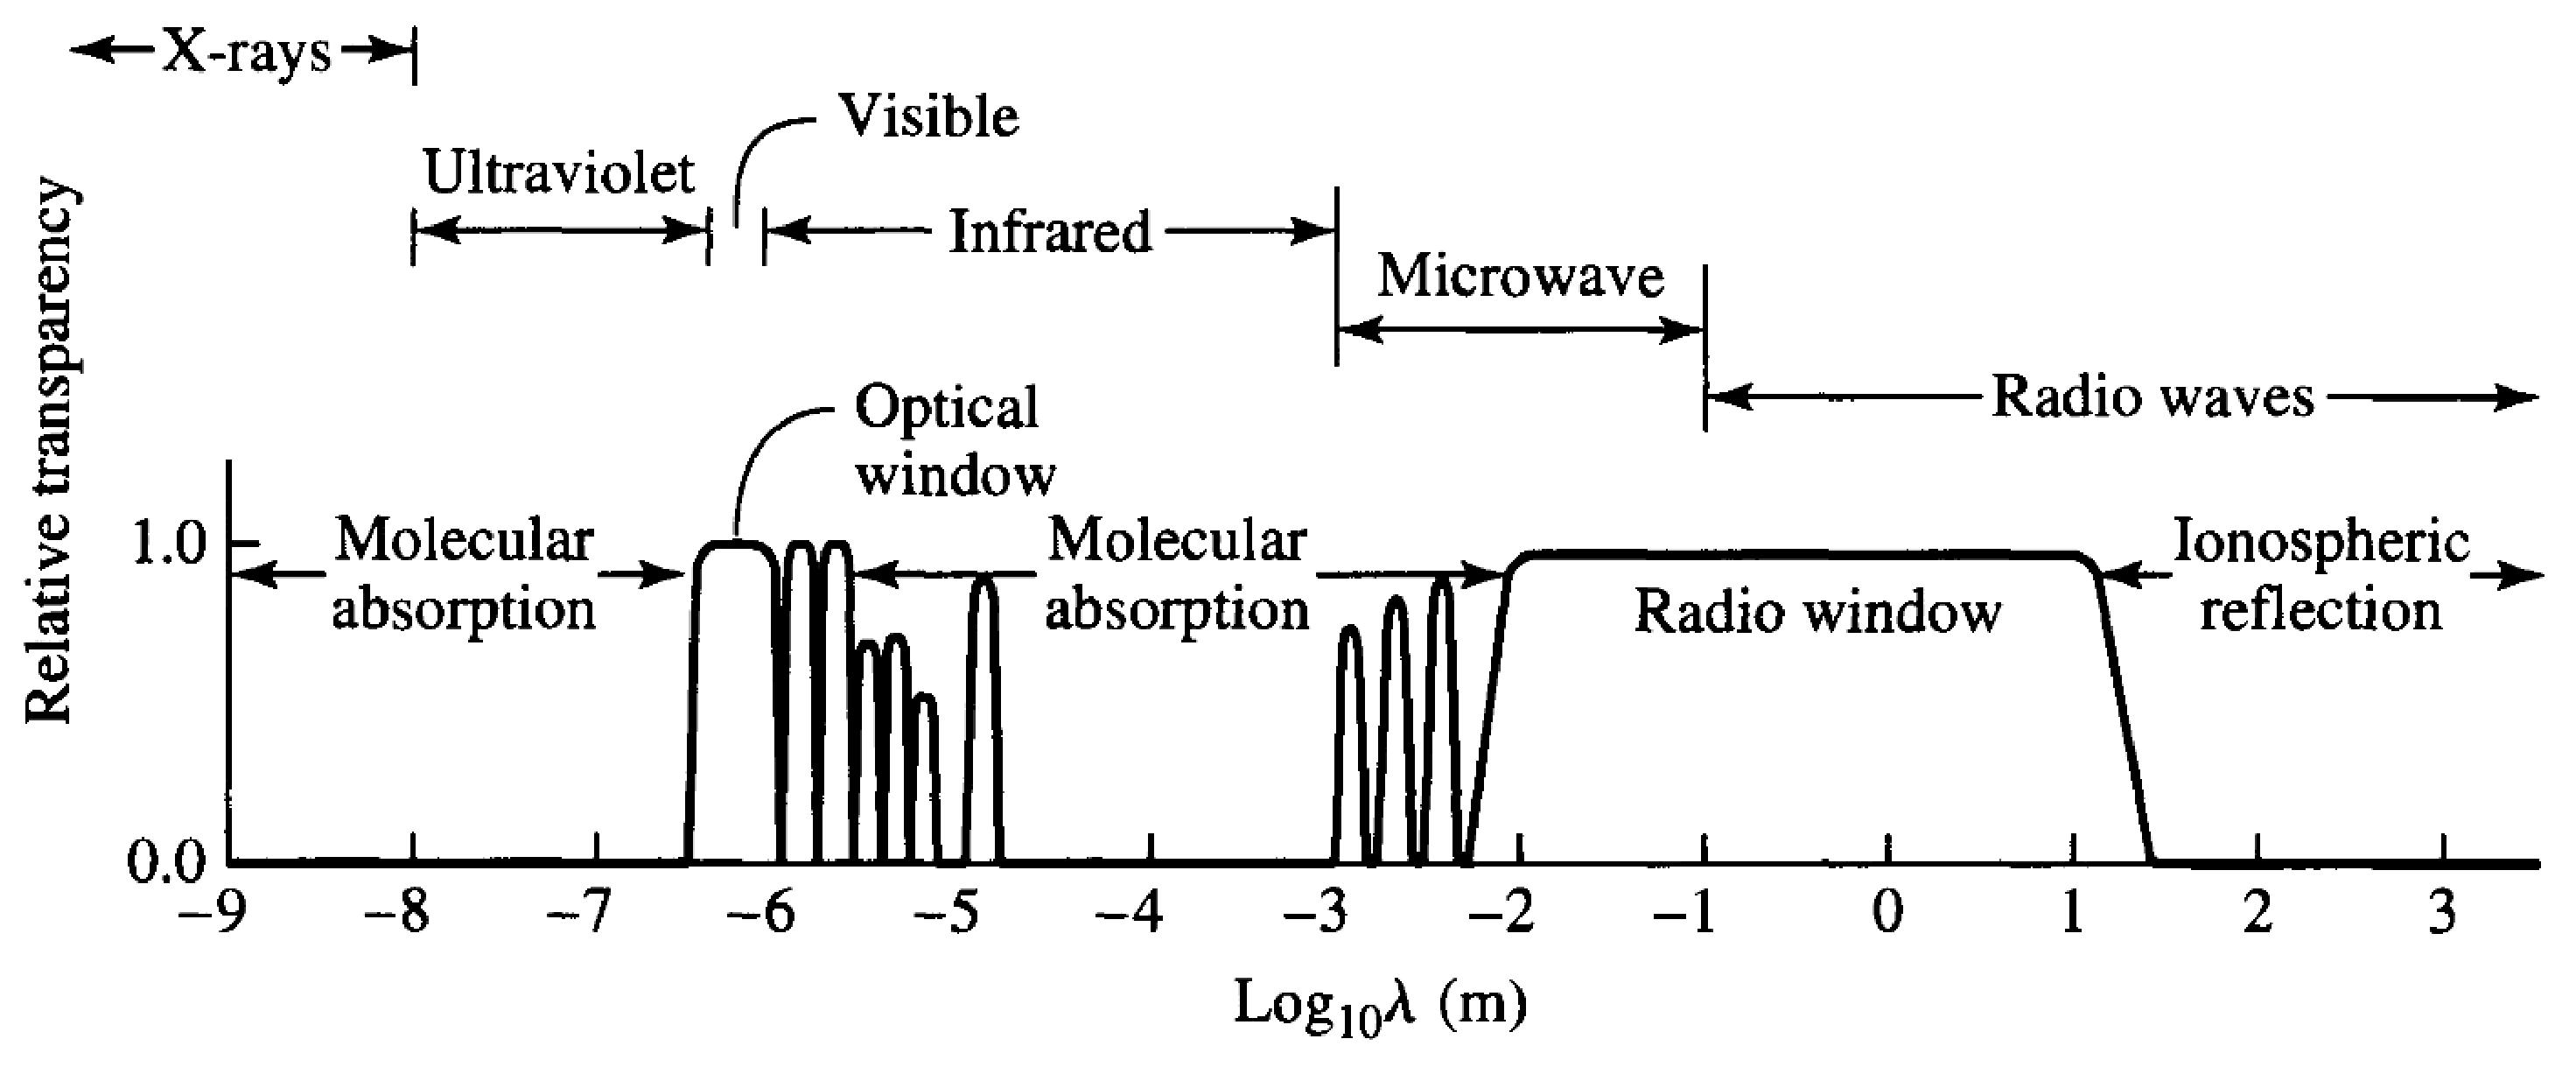
\includegraphics[width=\textwidth]{chapters/introduction/figures/atmospheric_absorption.pdf}
  \figlabel{atmospheric_absorption}
  \caption{
  Transparency of the atmosphere of the earth to photons of 
  varying wavelenthts.  This figure is from \cite{carroll_2006_introduction-modern}
  }
\end{figure}

% Thorough discussion of all experiments:
%   http://imagine.gsfc.nasa.gov/docs/sats_n_data/gamma_missions.html
%   http://space.about.com/od/telescopesandoptics/a/Gammaray-Astronomy.htm

% Nice history with lots of pictures:
%  http://fermi.gsfc.nasa.gov/science/mtgs/symposia/2012/program/mon/DKniffen.pdf

% Good books with introduction

%  "Very High Energy Gamma Ray Astronomy" by Trevor C. Weekes
%    * seems to have a discussion of the principles of Gamma-ray detection.
%      scintilation detectors, spark chambers.

%  "Cosmic Gamma-Ray Sources" - edited by K.S. Cheng, Gustavo E. Romero

% Very nice reference:
%   http://adsabs.harvard.edu/abs/1984BASI...12..202P

% Nice summary:
%   http://articles.adsabs.harvard.edu/cgi-bin/nph-iarticle_query?1984BASI...12..202P&amp;data_type=PDF_HIGH&amp;whole_paper=YES&amp;type=PRINTER&amp;filetype=.pdf

Astronomy has historically been almost entirely concerned with studying
the photons that arrive from outer space.  Because of their charge
neutrality, photons are not defected by intergalactic electric and
magnetic fields and therefore point back to the objects 
emitting them. 

Historically, the field of astronomy concerned
the study of visible light. The reason for this is visible light
is not signifcantly absorbed in the atmosphere. 
In addition to the visible spectrum, radio waves, some
energies of infrared radiation, and long-wavelenth ultraviolet
radiation can be measured from the ground. Figure
\figref{atmospheric_absorption} shows the transparancy
of the atmosphere of the earth to photons of differnet wavelenths.

Slowly, over time, astronomers expanded their view across the
electromagnetic spectrum.  First, the astronomical observations
were made from the ground.  Infrared radiation from the sun was
first observed by William Herschel in 1800. Herschel measured this
infrared radiation by measuring the temperature of sunlight through
a prisim and extending the measurement past the red part of the
spectrum \citep{herschel_1800_experiments-refrangibility}.  The first
extraterrestrial source of radio waves was detected by Jansky in 1933.
Janksy, a radio engineer at Bell labs, was studying the
origins of radio interference when he detected radio emission towards
the center of our galaxy.
\citep{jansky_1933_electrical-disturbances}.

% x-ray: http://en.wikiversity.org/wiki/Radiation_history#cite_ref-Burnight_183-1
The expansion of the astronomical fronteire to other wavelenths required
the development of rockets and sattelites in the 20th ceuntry.  The first
ultraviolet observation of the sun was performed in 1946 from a captured
V-2 rocket \citep{baum_1946_ultraviolet-spectrum}.  Observations of
solar x-rays were also first carried out on a captured V-2 Rocket in
1949 \citep{burnight_1949_x-radiation-atmosphere}.
